\documentclass[twocolumn,preprintnumbers,amsmath,amssymb,longbibliography]{revtex4-1}

\usepackage{graphicx}% Include figure files
\usepackage{dcolumn}% Align table columns on decimal point
\usepackage{bm}% bold math
\usepackage{float}
\usepackage{siunitx}

% Set one inch margins all around
\setlength\textwidth{6.5in}
\setlength\oddsidemargin{0in}
\setlength\evensidemargin{0in}

\setlength\textheight{9in}
\setlength\topmargin{-0.25in}
\setlength\headheight{0in}

\begin{document}

\title{Sand Timer Lab Report}% Force line breaks with \\

\author{Aether Zhou}
\affiliation{%
Department of Physics, University of California, Santa Barbara, CA 93106
}%

\date{\today}% It is always \today, today

\maketitle


\section{Experimental Methods}
In this experiment, two sand timers and one smartphone camera is used. We first set timers on an even table, wait for the sand flow stop, and shake timers gently to clear residual sand in the upper half. Then we turn on the camera, and flip sand timer A and B successively. After sand flow in both timers become invisible to naked eye, we turn off the camera, so the whole timing process is recorded. We repeated above procedures for 20 times, and from the 20 videos, we can get four essential data from each. By examining videos after the experiment, we can identify four essential frames each with a timestamp with precision $\pm 0.01$ second. 

For each trial, $(1)$ We flip the first timer by hand and keep the time duration between timer leave the table and back to the table as short as possible. When the timer appear horizontal to the table, we mark this frame as start point of a timing process. $(2)$ After we flip the first timer, we flip the second timer, and identify the `horizontal' frame for the second timer. $(3)$ When the sand flow becomes invisible to naked eye in one timer, we mark this frame as the end point of timing process of this timer. $(4)$ Mark another end point the same way as before. 


\begin{figure}[H]
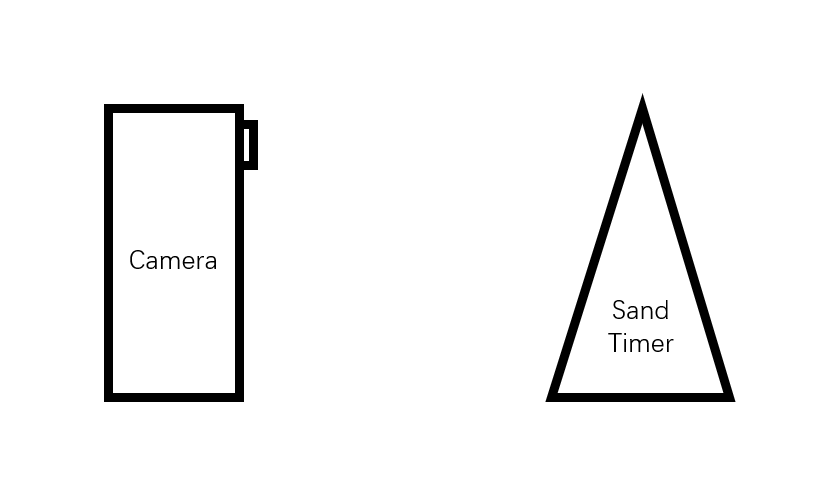
\includegraphics[width=3.5cm]{setting_1.png}
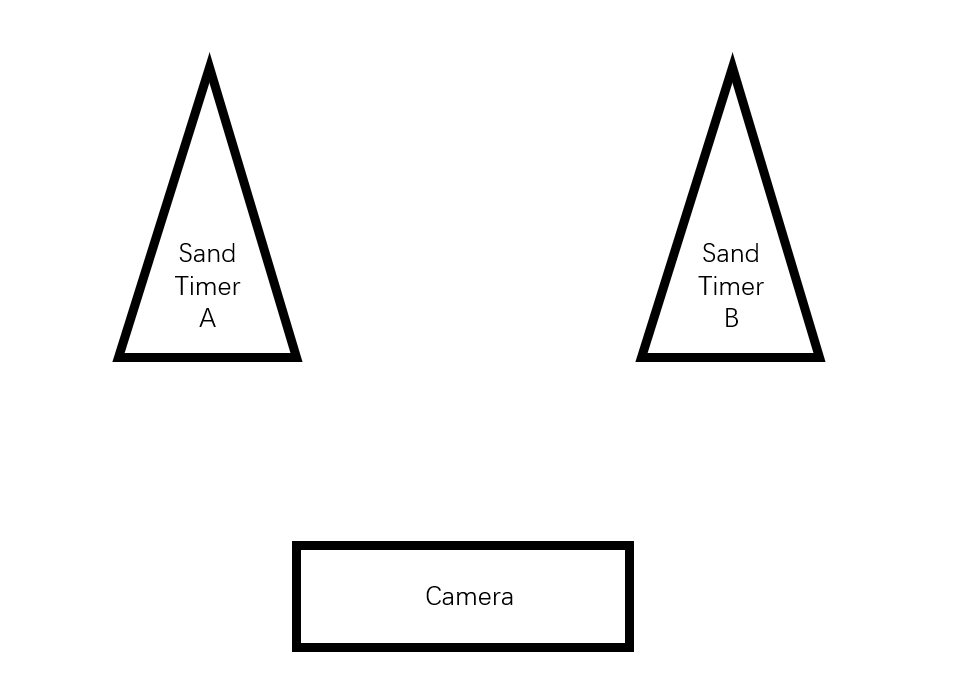
\includegraphics[width=4.3cm]{setting_2.png}
\caption{\label{setup} Setup of the sand timers. The left figure is the side view, and the right figure is the above view.} 
\end{figure}

Hence, for each video or each trail, we record the start and end point for timer A and timer B, four data in total. And we subtract end point timestamp by the corresponding start point timestamp to get the time duration `measured' by each sand timer. Also, we need to consider the difference between forward timing and backward timing, which can be caused by the symmetry break of sand timer due to structure defects. So we separate the videos into two groups: forward timing and backward timing. And for each group, we measure 10 time duration for each timer. 

\section{Data Analysis}
From our data, we can calculate the mean flow time for each timer. For sand timer A, the mean forward flow time is $56.45 (\pm 0.038)$ second, and the mean backward flow time is $57.37 (\pm 0.040)$ second; for sand timer B, the mean forward flow time is $61.16 (\pm 0.033)$ second, and the mean backward flow time is $57.06 (\pm 0.035)$ second.


\begin{figure}[H]
\centering
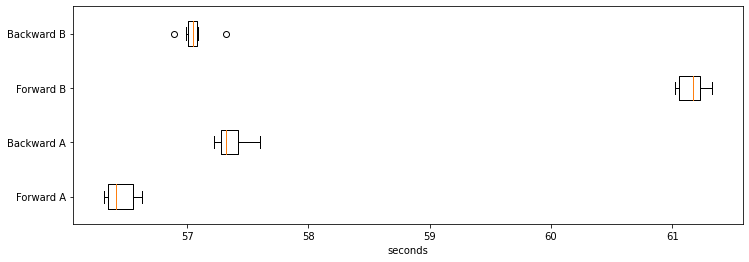
\includegraphics[width=8cm]{data.png}
\caption{\label{data} Time duration measured for each timer under forward mode and backward mode.} 
\end{figure}
    

For the forward timing case, sand timer B took 4.71 seconds more than timer A; for the backward timing case, sand timer B took 0.31 seconds less than timer A. Possible source of error may include precision of timestamp $(\pm 0.01 \si{.s})$ and frame rate of video taken $(30 \si{.fps})$. In general, timer A flows faster than timer B, this may due to structural difference (i.e. amount of sand). Also, timer B is flipped after timer A in all trails, so the action of flipping timer B might introduce perturbation to timer A, and make timer A flow faster in a certain time range. 

\section{Conclusions}
Statistical error is standard deviation over square root of number of trials, so it will decrease as we increase the number of measurement. Systematic error is related to equipment used (i.e. electric clock in phone), and we cannot reduce it by merely increasing trail number. If given more time and resources, we can design a flipping equipment to limit variables in the flipping process (reduce systematic error), and increase trial numbers (reduce statistical error).

\end{document}
%
% ****** End of file apssamp.tex ******
